\documentclass[11pt,a4paper]{article}

\usepackage[utf8]{inputenc}
\usepackage[T1]{fontenc}
\usepackage{amsmath,amssymb}
\usepackage{graphicx}
\usepackage{booktabs}
\usepackage{multirow}
\usepackage{xcolor}
\usepackage[hyphens]{url}
\usepackage{hyperref}
\expandafter\def\expandafter\UrlBreaks\expandafter{\UrlBreaks\do\/\do-\do_}
\usepackage{tikz}
\usetikzlibrary{shapes,arrows,positioning,fit,backgrounds}
\usepackage[margin=1in]{geometry}
\usepackage[numbers,sort&compress]{natbib}
\usepackage{longtable}
\usepackage{float}
\usepackage{listings}

\definecolor{botred}{RGB}{231,76,60}
\definecolor{hubblue}{RGB}{52,152,219}
\definecolor{organicgreen}{RGB}{46,204,113}
\definecolor{automatedorange}{RGB}{230,126,34}

\lstset{
    basicstyle=\ttfamily\small,
    breaklines=true,
    frame=single,
    backgroundcolor=\color{gray!10},
}

\title{\textbf{Supplementary Notes}\\[0.5em]
\large Tracking Dataset Reuse in Proteomics: A Comprehensive Analysis of PRIDE Archive Downloads}

\author{
\small Suresh Hewapathirana, Jingwen Bai, Chakradhar Bandla, Selvakumar Kamatchinathan,\\
\small Deepti J Kundu, Nithu Sara John, Boma Brown-Harry, Nandana Madhusoodanan,\\
\small Marc Riera Duocastella, Juan Antonio Vizca\'{i}no, Yasset Perez-Riverol
}
\date{}

\begin{document}
\maketitle

\tableofcontents
\newpage

% ======================================================================
\section{S1. Data Processing Pipeline}
\label{sec:pipeline}
% ======================================================================

\subsection{Log Processing Workflow}

PRIDE download logs are processed through the \texttt{nf-downloadstats} Nextflow pipeline (Figure~\ref{fig:pipeline_workflow}), which retrieves raw TSV log files, parses and filters download events, merges records into a consolidated Parquet file, and generates statistics reports. The pipeline produces a 4.7~GB Parquet file containing 159.3 million records optimized for columnar analytics.

\begin{figure}[H]
\centering
\includegraphics[width=0.8\textwidth]{figures/supp_pipeline_workflow.png}
\caption{The \texttt{nf-downloadstats} workflow for processing PRIDE download logs. Raw TSV logs are parsed, filtered, and merged into a Parquet file for efficient downstream analysis.}
\label{fig:pipeline_workflow}
\end{figure}

\subsection{Data Scale and Coverage}

The processed dataset covers the period January 2020 through January 2025 (Figure~\ref{fig:pride_overview}). Key metrics include 47.35 million total file downloads across 32,106 distinct projects, 2.26 million unique files, and 807,156 unique users. The analyzed projects represent 96.4\% of all public PRIDE datasets, and 88.0\% of PRIDE files have been downloaded at least once. Downloads originate from 136 countries with more than 100 downloads each.

\begin{figure}[H]
\centering
\includegraphics[width=\textwidth]{figures/supp_pride_overview.png}
\caption{Overview of PRIDE download activity (2020--2025). Overall scale metrics, reuse intensity across projects/files/users, file coverage, and geographic reach.}
\label{fig:pride_overview}
\end{figure}

% ======================================================================
\section{S2. Bot Detection Architecture}
\label{sec:architecture}
% ======================================================================

\subsection{System Overview}

DeepLogBot implements a multi-stage bot detection pipeline (Figure~\ref{fig:architecture_supp}) that processes download logs through feature extraction, anomaly detection, and hierarchical classification. The system supports two classification methods, each with distinct strengths.

\begin{figure}[H]
\centering
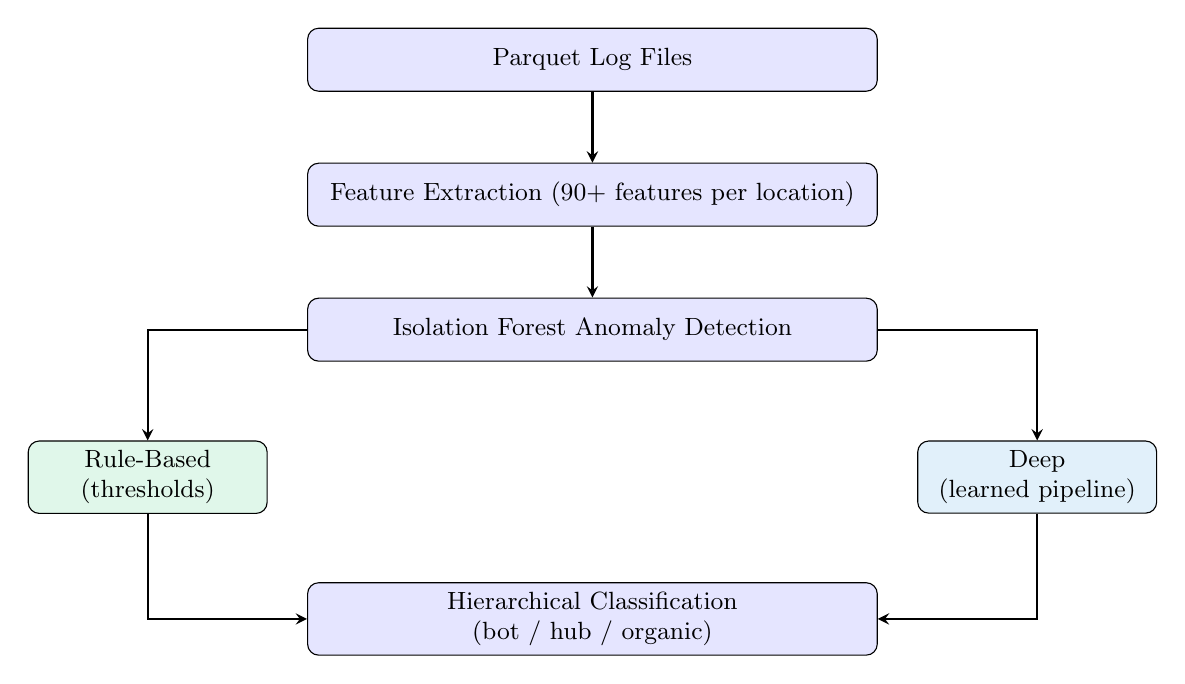
\begin{tikzpicture}[
    node distance=0.9cm,
    block/.style={rectangle, draw, fill=blue!10, text width=7cm, text centered, rounded corners, minimum height=0.8cm, font=\small},
    method/.style={rectangle, draw, rounded corners, minimum height=0.8cm, text centered, font=\small},
    arrow/.style={->, >=stealth, thick}
]
\node[block] (input) {Parquet Log Files};
\node[block, below=of input] (features) {Feature Extraction (90+ features per location)};
\node[block, below=of features] (anomaly) {Isolation Forest Anomaly Detection};

\node[method, below left=1cm and 0.5cm of anomaly, fill=organicgreen!15, text width=2.8cm] (rules) {Rule-Based\\(thresholds)};
\node[method, below right=1cm and 0.5cm of anomaly, fill=hubblue!15, text width=2.8cm] (deep) {Deep\\(learned pipeline)};

\node[block, below=2.8cm of anomaly] (output) {Hierarchical Classification\\(bot / hub / organic)};

\draw[arrow] (input) -- (features);
\draw[arrow] (features) -- (anomaly);
\draw[arrow] (anomaly) -| (rules);
\draw[arrow] (anomaly) -| (deep);
\draw[arrow] (rules) |- (output);
\draw[arrow] (deep) |- (output);
\end{tikzpicture}
\caption{DeepLogBot system architecture. Both methods share feature extraction and Isolation Forest anomaly detection; classification is performed by either a rule-based or learned deep pipeline.}
\label{fig:architecture_supp}
\end{figure}

% ======================================================================
\section{S3. Feature Catalog}
\label{sec:features}
% ======================================================================

DeepLogBot computes 90+ features per location, organized into six categories. Table~\ref{tab:all_features} provides the complete catalog.

\begin{longtable}{p{5.2cm}p{9.3cm}}
\caption{Complete feature catalog organized by category.}\label{tab:all_features}\\
\toprule
\textbf{Feature} & \textbf{Description} \\
\midrule
\endfirsthead
\toprule
\textbf{Feature} & \textbf{Description} \\
\midrule
\endhead
\multicolumn{2}{l}{\textit{\textbf{Basic Activity (21 features)}}} \\
\texttt{unique\_users} & Number of distinct user identifiers \\
\texttt{downloads\_per\_user} & Total downloads / unique users \\
\texttt{total\_downloads} & Aggregate download count \\
\texttt{projects\_per\_user} & Unique datasets / unique users \\
\texttt{avg\_users\_per\_hour} & Average unique users across active hours \\
\texttt{max\_users\_per\_hour} & Peak unique users in any single hour \\
\texttt{user\_cv} & Coefficient of variation of users per hour \\
\texttt{users\_per\_active\_hour} & Users per hour (only counting active hours) \\
\texttt{hourly\_download\_std} & Standard deviation of hourly download counts \\
\texttt{peak\_hour\_concentration} & Fraction of downloads in the busiest hour \\
\texttt{working\_hours\_ratio} & Fraction during 9AM--6PM local time \\
\texttt{hourly\_entropy} & Shannon entropy of hourly distribution \\
\texttt{night\_activity\_ratio} & Fraction during 10PM--6AM \\
\texttt{yearly\_entropy} & Distribution uniformity across years \\
\texttt{peak\_year\_concentration} & Max year's fraction of all downloads \\
\texttt{years\_span} & Number of years with activity \\
\texttt{downloads\_per\_year} & Average annual download count \\
\texttt{year\_over\_year\_cv} & CV of yearly download counts \\
\texttt{fraction\_latest\_year} & Latest year's share of total \\
\texttt{is\_new\_location} & Binary: only active in latest year \\
\texttt{spike\_ratio} & Latest year / historical average \\
\midrule
\multicolumn{2}{l}{\textit{\textbf{Advanced Behavioral (15 features)}}} \\
\texttt{burst\_pattern\_score} & Concentration of downloads in short time windows \\
\texttt{circadian\_rhythm\_deviation} & Deviation from typical human circadian patterns \\
\texttt{user\_coordination\_score} & Synchronized activity across user IDs \\
\texttt{hourly\_cv\_burst} & CV of hourly counts (burst detection) \\
\texttt{spike\_intensity} & Magnitude of download spikes \\
\texttt{user\_peak\_ratio} & Peak-hour users / average users \\
\texttt{night\_ratio\_advanced} & Refined night activity metric \\
\texttt{work\_ratio\_advanced} & Refined working hours metric \\
\texttt{evening\_ratio} & 6PM--10PM activity fraction \\
\texttt{morning\_ratio} & 6AM--9AM activity fraction \\
\texttt{user\_coordination\_std} & Variability in coordination patterns \\
\texttt{avg\_concurrent\_users} & Average concurrent active users \\
\texttt{max\_concurrent\_users} & Peak concurrent users \\
\texttt{is\_bursty\_advanced} & Binary: exhibits burst patterns \\
\texttt{is\_nocturnal} & Binary: predominantly night activity \\
\midrule
\multicolumn{2}{l}{\textit{\textbf{Bot Interaction (6 features)}}} \\
\texttt{dl\_user\_per\_log\_users} & Downloads per user normalized by log(users) \\
\texttt{user\_scarcity\_score} & Inverse user density measure \\
\texttt{download\_concentration} & Gini of download distribution across users \\
\texttt{temporal\_irregularity} & Non-uniformity of temporal access patterns \\
\texttt{bot\_composite\_score} & Weighted combination of bot indicators \\
\texttt{anomaly\_dl\_interaction} & Anomaly score $\times$ download concentration \\
\midrule
\multicolumn{2}{l}{\textit{\textbf{Bot Signature (8 features)}}} \\
\texttt{request\_velocity} & Downloads per active day \\
\texttt{access\_regularity} & Regularity of access intervals \\
\texttt{ua\_per\_user} & User agent diversity per user \\
\texttt{ip\_concentration} & IP address concentration \\
\texttt{session\_anomaly} & Deviation from normal session patterns \\
\texttt{request\_pattern\_anomaly} & Unusual request sequences \\
\texttt{weekend\_weekday\_imbalance} & Weekend vs weekday activity ratio \\
\texttt{is\_high\_velocity} & Binary: extremely high request rate \\
\midrule
\multicolumn{2}{l}{\textit{\textbf{Discriminative (17 features)}}} \\
\texttt{file\_exploration\_score} & Breadth of file access patterns \\
\texttt{file\_mirroring\_score} & Consistency with mirroring behavior \\
\texttt{file\_entropy} & Shannon entropy of file access distribution \\
\texttt{bot\_farm\_score} & User homogeneity (coordinated fakes) \\
\texttt{user\_authenticity\_score} & Diversity of user behavior patterns \\
\texttt{user\_homogeneity\_score} & Similarity across users at location \\
\texttt{geographic\_stability} & IP geographic consistency \\
\texttt{version\_concentration} & Concentration in file versions \\
\texttt{targets\_latest\_only} & Binary: only accesses latest versions \\
\texttt{unique\_versions} & Number of distinct file versions \\
\texttt{lifespan\_days} & Duration of activity \\
\texttt{activity\_density} & Active days / total lifespan \\
\texttt{persistence\_score} & Long-term consistent access pattern \\
\texttt{malicious\_bot\_score} & Composite malicious indicator \\
\texttt{legitimate\_auto\-mation\_score} & Composite legitimate indicator \\
\texttt{bot\_vs\_legit\-imate\_score} & Differential (malicious $-$ legitimate) \\
\texttt{is\_likely\_malicious} & Binary: likely malicious automation \\
\midrule
\multicolumn{2}{l}{\textit{\textbf{Time Series (23 features)}}} \\
\multicolumn{2}{l}{\textit{Outburst Detection (6 features)}} \\
\texttt{outburst\_count} & Number of spikes ($>2$ standard deviations) \\
\texttt{outburst\_intensity} & Average spike magnitude \\
\texttt{max\_outburst\_zscore} & Highest Z-score across time windows \\
\texttt{outburst\_ratio} & Fraction of activity in outbursts \\
\texttt{time\_since\_last\_outburst} & Recency of latest spike \\
\texttt{longest\_outburst\_streak} & Max consecutive high-activity periods \\
\midrule
\multicolumn{2}{l}{\textit{Periodicity Detection (4 features)}} \\
\texttt{weekly\_autocorr} & Autocorrelation at 7-day lag \\
\texttt{dominant\_period\_days} & Most significant period (FFT) \\
\texttt{periodicity\_strength} & Strength of dominant period \\
\texttt{period\_regularity} & Consistency of the period \\
\midrule
\multicolumn{2}{l}{\textit{Trend Analysis (5 features)}} \\
\texttt{trend\_slope} & Linear trend direction (normalized) \\
\texttt{trend\_strength} & $R^2$ of linear fit \\
\texttt{trend\_acceleration} & Second derivative \\
\texttt{detrended\_volatility} & Volatility after removing trend \\
\texttt{trend\_direction} & Categorical ($-1$, $0$, $+1$) \\
\midrule
\multicolumn{2}{l}{\textit{Recency-Weighted (4 features)}} \\
\texttt{recent\_activity\_ratio} & Recent 30 days vs historical average \\
\texttt{recent\_volatility\_ratio} & Recent CV vs historical CV \\
\texttt{recency\_concentration} & Fraction in last 30 days \\
\texttt{momentum\_score} & Exponentially-weighted trend \\
\midrule
\multicolumn{2}{l}{\textit{Bot Signature Temporal (3 features)}} \\
\texttt{autocorrelation\_lag1} & Day-to-day correlation \\
\texttt{circadian\_deviation} & Distance from human circadian pattern \\
\texttt{request\_timing\_entropy} & Entropy of request timing \\
\bottomrule
\end{longtable}

% ======================================================================
\section{S4. Algorithm Details}
\label{sec:algorithms}
% ======================================================================

\subsection{Rule-Based Method}

The rule-based method applies threshold patterns from a YAML configuration file. Classification proceeds top-down through three levels:

\begin{sloppypar}
\begin{enumerate}
    \item \textbf{Level~1 (Behavior Type):} Organic patterns match on \texttt{working\_hours\_ratio}~$\geq 0.4$ and \texttt{regularity\_score}~$\leq 0.6$, or \texttt{interval\_cv}~$\geq 0.7$, or \texttt{unique\_users}~$< 50$ with moderate activity. Automated patterns match on \texttt{regularity\_score}~$\geq 0.7$, or \texttt{night\_activity\_ratio}~$\geq 0.35$ with low working hours, or \texttt{user\_coordination\_score}~$\geq 0.6$ with many users.

    \item \textbf{Level~2 (Automation Category):} Bot patterns include many-users-low-downloads (\texttt{unique\_users}~$\geq 1000$, \texttt{downloads\_per\_user}~$\leq 50$), coordinated activity (\texttt{coordination\_score}~$\geq 0.7$, \texttt{authenticity\_score}~$\leq 0.4$), and suspicious timing (\texttt{night\_activity\_ratio}~$\geq 0.5$, \texttt{working\_hours\_ratio}~$\leq 0.2$). Legitimate automation matches on mirror patterns (\texttt{downloads\_per\_user}~$\geq 500$, \texttt{unique\_users}~$\leq 100$) or CI/CD patterns (\texttt{users}~$\leq 10$, \texttt{regularity}~$\geq 0.7$).

    \item \textbf{Level~3 (Subcategory):} Nine subcategories provide granular classification within each automation category.
\end{enumerate}
\end{sloppypar}

\subsection{Deep Architecture Method}

The deep method implements a five-stage learned pipeline that replaces hand-tuned thresholds with data-driven decisions:

\begin{enumerate}
    \item \textbf{Seed Selection.} High-confidence organic, bot, and hub locations are identified from feature distributions (e.g., download-per-user thresholds, working hours ratio). These seeds provide training labels for downstream stages.

    \item \textbf{Organic VAE.} A variational autoencoder is trained on organic seed locations to learn the manifold of normal download behavior. Locations with high reconstruction error are flagged as anomalous.

    \item \textbf{Deep Isolation Forest.} Non-linear anomaly detection via neural projections (DeepOD library, with scikit-learn Isolation Forest as fallback) captures complex anomaly patterns in the feature space.

    \item \textbf{Temporal Consistency.} Modified z-score spike detection without fixed thresholds identifies temporal anomalies by comparing each location's download patterns against robust statistical baselines.

    \item \textbf{Fusion Meta-Learner.} A gradient-boosted classifier combines all anomaly signals---VAE reconstruction error, deep IF scores, temporal anomaly scores, and 33 behavioral features---into calibrated three-class probabilities (bot/hub/organic) via Platt scaling.
\end{enumerate}

\begin{sloppypar}
Additionally, soft priors encode pre-filter signals as continuous features (no hard lockout), and a reconciliation step overrides predictions when the pipeline and pre-filter strongly disagree. Post-classification stages include hub protection (preventing legitimate automation from being misclassified as bots) and detailed subcategory assignment.
\end{sloppypar}


% ======================================================================
\section{S5. Ground Truth Construction}
\label{sec:ground_truth}
% ======================================================================

Ground truth labels were assigned using high-confidence heuristic criteria applied to a 1-million record sample (Table~\ref{tab:ground_truth}):

\begin{table}[H]
\centering
\caption{Ground truth label criteria and counts.}
\label{tab:ground_truth}
\small
\begin{tabular}{llrp{6cm}}
\toprule
\textbf{Label} & \textbf{Subtype} & \textbf{Count} & \textbf{Criteria} \\
\midrule
\multirow{3}{*}{Bot} & Ground truth bot & -- & $\geq$10K users, $\leq$10 DL/user \\
& Large-scale bot & -- & $\geq$5K users, $\leq$25 DL/user \\
& Bot farm & -- & $\geq$1K users, $\leq$50 DL/user, work ratio $\leq$0.3 \\
\cmidrule{2-4}
& \textbf{Total} & \textbf{88} & \\
\midrule
\multirow{3}{*}{Hub} & Mirror & -- & $\leq$5 users, $\geq$1K DL/user \\
& Institutional hub & -- & $\leq$20 users, $\geq$500 DL/user \\
& Research hub & -- & 10--200 users, $\geq$200 DL/user, $\geq$100K total, work ratio $\geq$0.2 \\
\cmidrule{2-4}
& \textbf{Total} & \textbf{44} & \\
\midrule
\multirow{3}{*}{Organic} & Individual user & -- & $\leq$3 users, $\leq$20 DL/user, work ratio $\geq$0.4 \\
& Research group & -- & 3--30 users, 5--100 DL/user, work ratio $\geq$0.35 \\
& Casual user & -- & $\leq$5 users, $\leq$50 DL/user, night ratio $\leq$0.3 \\
\cmidrule{2-4}
& \textbf{Total} & \textbf{1,279} & \\
\midrule
Uncertain & -- & 18,634 & Excluded from benchmark \\
\bottomrule
\end{tabular}
\end{table}

% ======================================================================
\section{S6. Benchmark Details}
\label{sec:benchmark}
% ======================================================================

\subsection{Per-Category Performance}

Figure~\ref{fig:benchmark_heatmaps} shows precision, recall, and F1 per category for each method. The Rules method achieves the highest bot precision (0.506) but low hub recall (0.159). The Deep method balances all categories, with high hub precision (0.824) and the best hub recall (0.636).

\begin{figure}[H]
\centering
\includegraphics[width=\textwidth]{figures/supp_benchmark_heatmaps.pdf}
\caption{Per-category precision, recall, and F1 scores for each detection method.}
\label{fig:benchmark_heatmaps}
\end{figure}

\subsection{Bootstrap Confidence Intervals}

Macro F1 scores with 1,000-iteration bootstrap 95\% confidence intervals (Figure~\ref{fig:bootstrap_ci}): Deep achieves 0.775 [0.731, 0.818] and Rules achieves 0.632 [0.574, 0.691]. The non-overlapping CIs confirm a statistically significant performance difference between the two methods.

\begin{figure}[H]
\centering
\includegraphics[width=0.85\textwidth]{figures/supp_bootstrap_ci.pdf}
\caption{Macro F1 scores with 95\% bootstrap confidence intervals for both methods.}
\label{fig:bootstrap_ci}
\end{figure}

\subsection{Statistical Significance}

McNemar's test with continuity correction was used to compare methods pairwise (Table~\ref{tab:mcnemar}):

\begin{table}[H]
\centering
\caption{Pairwise McNemar's test results.}
\label{tab:mcnemar}
\begin{tabular}{lccc}
\toprule
\textbf{Comparison} & $\chi^2$ & \textbf{p-value} & \textbf{Significant?} \\
\midrule
Rules vs Deep & 0.024 & 0.877 & No \\
\bottomrule
\end{tabular}
\end{table}

Rules and Deep do not differ significantly ($p = 0.877$).

\subsection{Inter-Method Agreement}

Figure~\ref{fig:agreement_supp} shows pairwise agreement between methods. Rules and Deep agree on 87.8\% of classifications (Cohen's $\kappa$ = 0.508), indicating moderate agreement. Per-category agreement is highest for organic classification and lowest for hubs.

\begin{figure}[H]
\centering
\includegraphics[width=\textwidth]{figures/supp_figure_agreement.pdf}
\caption{Inter-method agreement analysis. (A) Pairwise overall agreement matrix. (B) Per-category agreement across method pairs.}
\label{fig:agreement_supp}
\end{figure}

\subsection{Classification Outcome Comparison}

On the 1M-record benchmark sample, the two methods produce different classification distributions (Figure~\ref{fig:method_comparison}). The Rules method classifies 29\% of locations as bots (72\% of downloads), while Deep classifies 34\% (77\% of downloads).

\begin{figure}[H]
\centering
\includegraphics[width=\textwidth]{figures/supp_method_comparison.pdf}
\caption{Classification outcome comparison. (A) Percentage of locations classified in each category. (B) Percentage of downloads attributed to each category.}
\label{fig:method_comparison}
\end{figure}

% ======================================================================
\section{S7. Bot Removal Analysis}
\label{sec:bot_removal}
% ======================================================================

\subsection{Full-Dataset Classification}

The Deep method---the best-performing algorithm in our benchmark (macro F1 = 0.775)---was applied to the complete dataset of 71,133 locations aggregated from 159.3 million download records. The classification results are summarized in Figure~\ref{fig:classification_dist}:

\begin{itemize}
    \item \textbf{Bot:} 37,779 locations (53.1\%), accounting for 88.0\% of downloads
    \item \textbf{Hub:} 664 locations (0.9\%), accounting for 11.3\% of downloads (institutional mirrors/aggregators)
    \item \textbf{Organic:} 32,690 locations (46.0\%), accounting for 0.7\% of downloads (genuine individual users)
\end{itemize}

\begin{figure}[H]
\centering
\includegraphics[width=\textwidth]{figures/supp_classification_distribution.pdf}
\caption{Full-dataset classification results. (A) Location distribution: roughly equal numbers of bot and organic locations. (B) Download distribution: bots generate 88.0\% of all traffic despite representing 53.1\% of locations.}
\label{fig:classification_dist}
\end{figure}

The asymmetry between location counts and download volumes is striking: bots generate far more traffic per location on average, while institutional hubs---though comprising only 0.9\% of locations---account for 11.3\% of all download volume.

\subsection{Geographic Impact of Bot Removal}

Bot removal changes the apparent geographic distribution of PRIDE usage (Figure~\ref{fig:bot_geographic}). After removing bot locations, the United States leads with 5.1M downloads (26.8\%), followed by the United Kingdom (4.5M, 23.6\%) and Germany (4.3M, 22.5\%). China, which dominates raw download volume before filtering, drops to sixth position (464K, 2.4\%) after bot removal, indicating that the vast majority of traffic from Chinese IP addresses was automated. Similarly, countries like Brazil and Hong Kong show significant decreases after filtering, confirming that much of their raw traffic was bot-generated.

\begin{figure}[H]
\centering
\includegraphics[width=\textwidth]{figures/supp_bot_removal_geographic.pdf}
\caption{Geographic distribution before and after bot removal. (A) Raw download counts dominated by bot traffic from East Asian locations. (B) After bot removal, the United States and Germany lead genuine usage.}
\label{fig:bot_geographic}
\end{figure}

% ======================================================================
\section{S8. Extended Usage Analysis}
\label{sec:extended}
% ======================================================================

\subsection{Monthly Download Trends}

Monthly download patterns (after bot removal) reveal temporal structure within the yearly trends (Figure~\ref{fig:monthly_trends}). Activity shows seasonal variation with increased downloads during the academic year and a notable surge in early 2025, likely reflecting both genuine growth and the inclusion of January 2025 data.

\begin{figure}[H]
\centering
\includegraphics[width=\textwidth]{figures/supp_monthly_trends.pdf}
\caption{Monthly download volume (after bot removal), showing seasonal patterns and overall growth.}
\label{fig:monthly_trends}
\end{figure}

\subsection{Hourly Activity Patterns}

Hourly download patterns (Figure~\ref{fig:hourly_patterns}) after bot removal show clear circadian rhythms consistent with human usage: peak activity occurs during daytime hours (UTC), with reduced activity during nighttime and weekends. This pattern validates the bot removal process, as genuine human users exhibit regular circadian behavior while bots typically show more uniform 24/7 activity.

\begin{figure}[H]
\centering
\includegraphics[width=0.75\textwidth]{figures/supp_hourly_patterns.pdf}
\caption{Download activity heatmap by hour (UTC) and day of week, after bot removal. The circadian pattern confirms genuine human usage.}
\label{fig:hourly_patterns}
\end{figure}

\subsection{Regional Distribution}

\begin{figure}[H]
\centering
\includegraphics[width=0.65\textwidth]{figures/figure1b_regional_distribution.pdf}
\caption{PRIDE downloads by world region (after bot removal, 2020--2025).}
\label{fig:regional_supp}
\end{figure}

\subsection{Protocol Distribution}

Across the entire study period, FTP accounts for 52.6\% of genuine downloads and HTTP for 46.0\% (Figure~\ref{fig:protocol_overall}). High-performance protocols are emerging: Aspera (FASP) accounts for 0.9\% of non-bot downloads and Globus for 0.5\%, indicating early but growing institutional adoption of high-throughput transfer tools.

\begin{figure}[H]
\centering
\includegraphics[width=0.7\textwidth]{figures/supp_protocol_overall.pdf}
\caption{Overall download method distribution across the study period (after bot removal).}
\label{fig:protocol_overall}
\end{figure}

\subsection{pridepy Adoption}

\begin{sloppypar}
To facilitate adoption of high-performance download protocols, the PRIDE team released \texttt{pridepy} \citep{Kamatchinathan2025}, a Python command-line tool that abstracts protocol complexity and enables seamless switching between FTP, Aspera, and Globus transfers. The package was published on PyPI in March 2025. Figure~\ref{fig:pridepy_downloads} shows the monthly download trend throughout 2025, with a total of 6,504 installations. Notably, downloads surged in October 2025 (1,111 installations), coinciding with the rapid growth of Aspera-based transfers observed in the PRIDE download logs (Figure~6B in the main text). This temporal correlation between \texttt{pridepy} adoption and Aspera usage growth supports the hypothesis that user-friendly tooling can lower barriers to high-performance protocol adoption in scientific data repositories.
\end{sloppypar}

\begin{figure}[H]
\centering
\includegraphics[width=0.85\textwidth]{figures/supp_pridepy_downloads.pdf}
\caption{Monthly PyPI download statistics for \texttt{pridepy} throughout 2025. The red bar marks the publication month (March 2025). The green line shows cumulative downloads. Data source: pypistats.org (August--December 2025) and ClickPy/ClickHouse (January--July 2025).}
\label{fig:pridepy_downloads}
\end{figure}

\subsection{Top Downloaded Datasets}

The top 20 most downloaded PRIDE datasets are shown in Figure~\ref{fig:top_datasets_supp}. The most downloaded dataset (PXD004732) has accumulated 355,082 downloads, while PXD017052 reaches the broadest geographic spread (103 countries). Several of the top datasets are large-scale reference proteome studies that serve as benchmarks in the community. Note that dataset rankings depend on the bot detection algorithm applied; the rankings shown here are based on the Deep method.

\begin{figure}[H]
\centering
\includegraphics[width=0.85\textwidth]{figures/figure6_top_datasets.pdf}
\caption{Top 20 most downloaded PRIDE datasets after bot removal, showing download volume and geographic reach.}
\label{fig:top_datasets_supp}
\end{figure}

\subsection{Dataset Download Consistency}

The consistency heatmap (Figure~7B in the main text) shows that top datasets maintain sustained download activity across multiple years rather than one-time spikes. Beyond this, we rank datasets by a consistency score combining low coefficient of variation with high activity ratio (Figure~\ref{fig:consistency_scores}). PXD013868 achieves the highest consistency score (0.788), indicating steady, reliable reuse across the study period.

\begin{figure}[H]
\centering
\includegraphics[width=0.85\textwidth]{figures/supp_consistency_scores.pdf}
\caption{Top 20 most consistently downloaded PRIDE datasets, ranked by consistency score = $(1 - \text{CV}) \times \text{activity ratio}$.}
\label{fig:consistency_scores}
\end{figure}

\subsection{File-Level Download Distribution}

At the individual file level, downloads follow a log-normal distribution (Figure~\ref{fig:downloads_per_file}), with most files receiving between 3 and 30 downloads. A small number of files exceed 1,000 downloads, representing benchmark datasets and popular reference proteomes.

\begin{figure}[H]
\centering
\includegraphics[width=0.6\textwidth]{figures/supp_downloads_per_file.pdf}
\caption{Distribution of downloads per file (log scale). The majority of files receive between 3--30 downloads.}
\label{fig:downloads_per_file}
\end{figure}

\subsection{Country-Level Usage Intensity}

The relationship between unique users and total downloads per country reveals distinct usage patterns (Figure~\ref{fig:bubble_chart}). Countries cluster along a diagonal indicating proportional usage, while some outliers show disproportionately high downloads per user (suggesting institutional bulk access) or many users with moderate downloads (widespread individual adoption). Bubble size and color represent downloads per user, highlighting intensity differences.

\begin{figure}[H]
\centering
\includegraphics[width=\textwidth]{figures/supp_bubble_chart.pdf}
\caption{Total downloads vs.\ unique users per country (log-log scale, after bot removal). Bubble size and color indicate downloads per user. Top 50 countries with $>$10,000 downloads shown.}
\label{fig:bubble_chart}
\end{figure}

\subsection{ProteomeXchange Resources}

PRIDE hosts 83.2\% of all ProteomeXchange datasets, followed by MassIVE (6.9\%) and iProX (5.5\%) (Figure~\ref{fig:px_resources}). This dominance reflects PRIDE's position as the primary public repository for mass spectrometry proteomics data.

\begin{figure}[H]
\centering
\includegraphics[width=0.5\textwidth]{figures/supp_px_resources.png}
\caption{Distribution of datasets across ProteomeXchange partner resources.}
\label{fig:px_resources}
\end{figure}

% ======================================================================
\section{S9. Limitations}
\label{sec:limitations}
% ======================================================================

Our ground truth labels are heuristic-derived rather than manually verified, which may introduce systematic biases in the benchmark evaluation. The geographic attribution relies on IP geolocation, which can be inaccurate for users behind VPNs or institutional proxies. The 2025 data is from a partial year, making year-over-year comparisons with full years approximate. Finally, we cannot distinguish multiple individual users who share a geographic location from a single user, which may affect location-level statistics.

\bibliographystyle{unsrtnat}
\bibliography{references}

\end{document}
